\subsection{Curve in funzione della pressione}
\FloatBarrier

\begin{grafico}
 \centering
 \resizebox{\textwidth}{!}{%
 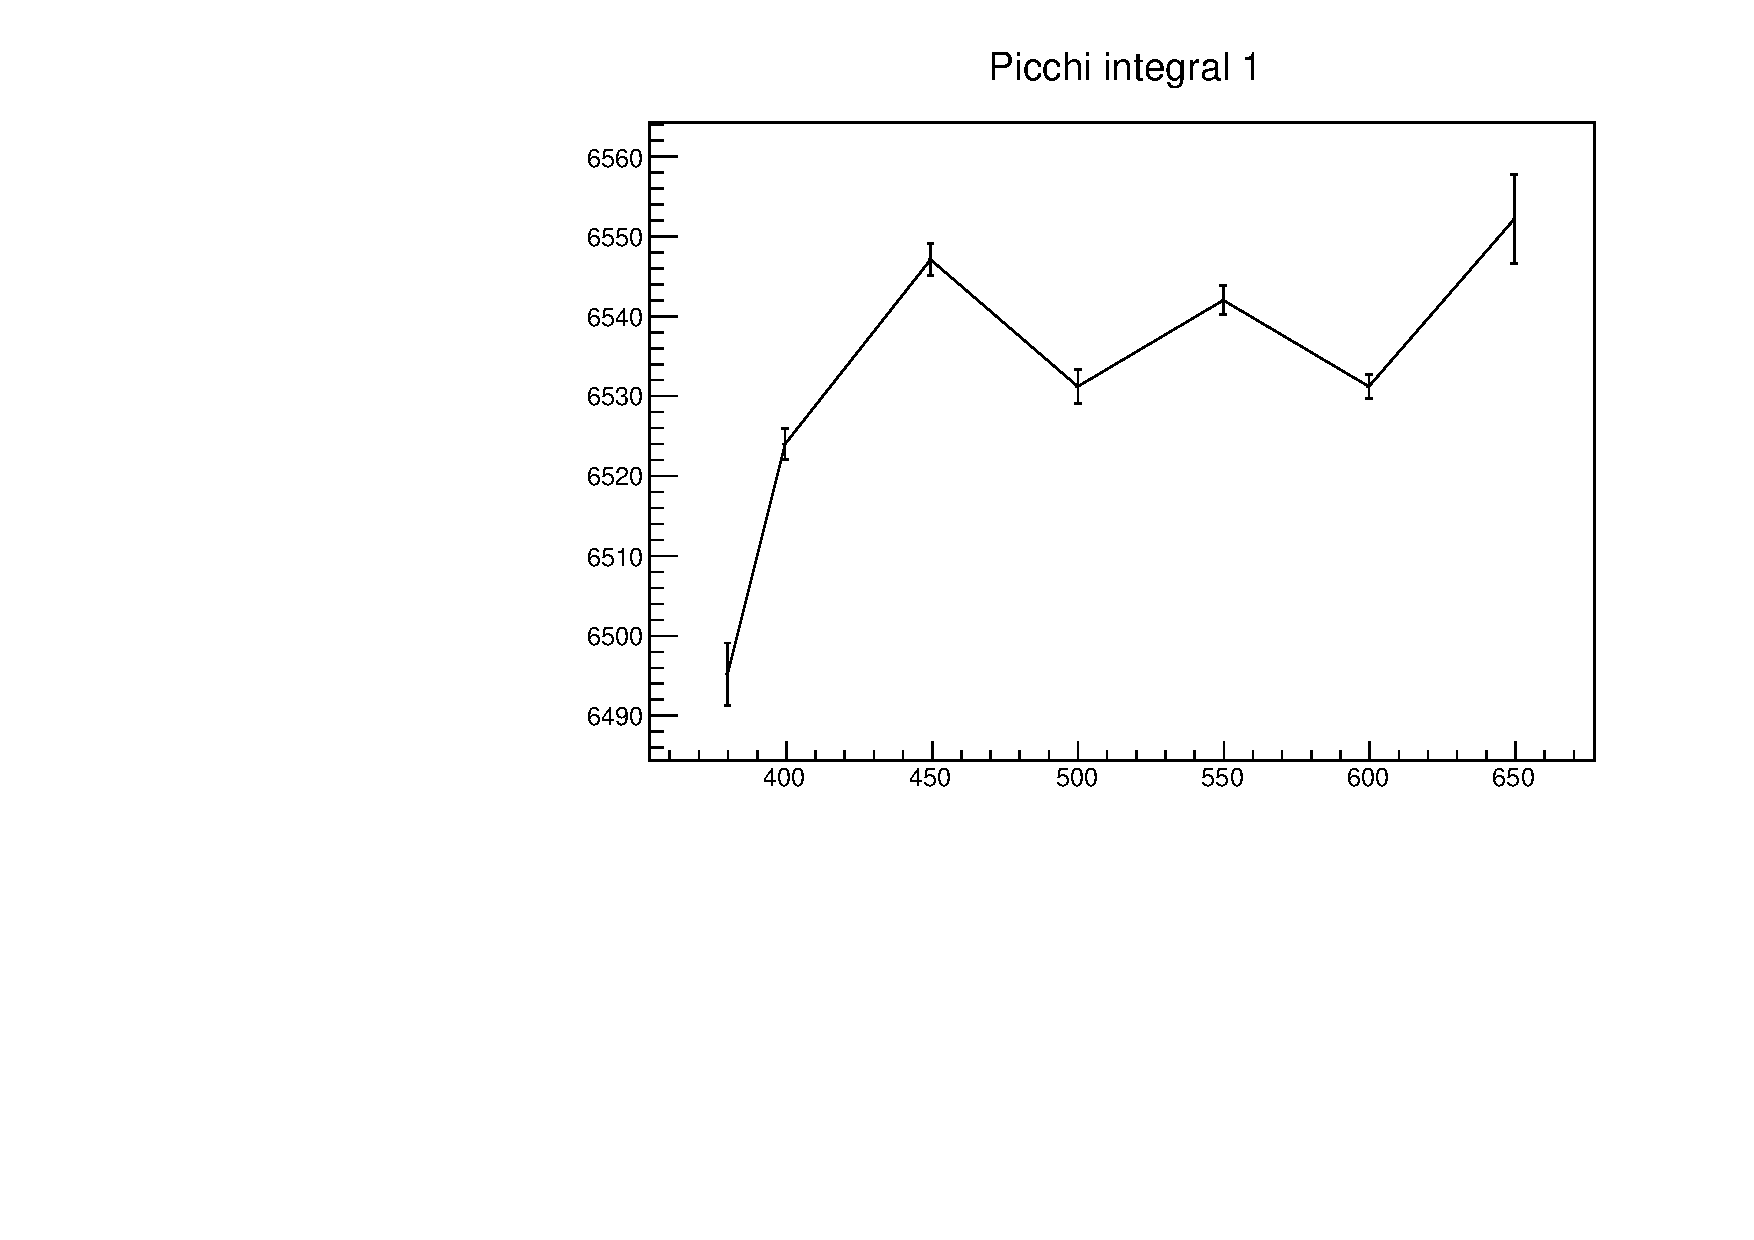
\includegraphics{../grafici/risultati/picchi_integral1.pdf}
 }%
 \caption{Andamento integrale del picco 1 in funzione della pressione [mb]} 
 \label{gr:picchi_int1} 
\end{grafico}

\begin{grafico}
 \centering
 \resizebox{\textwidth}{!}{%
 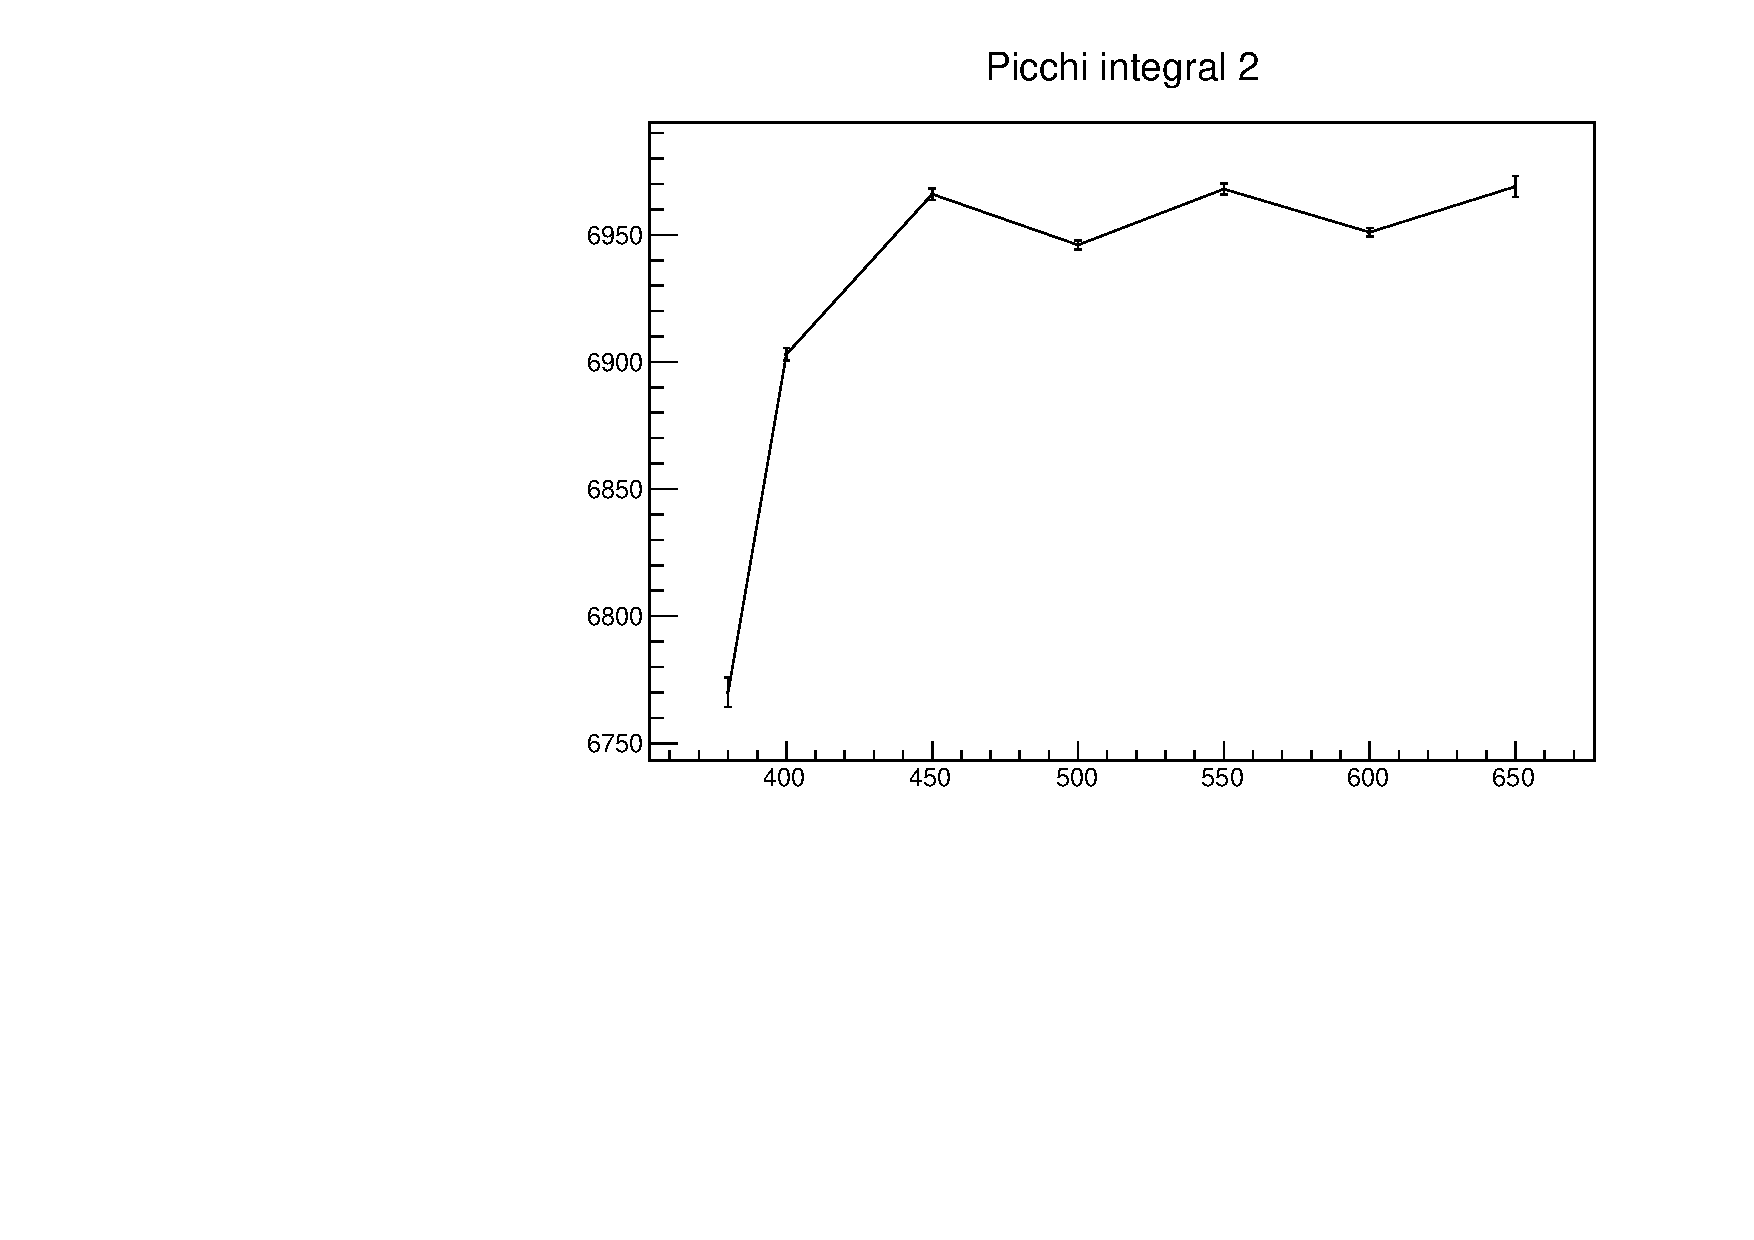
\includegraphics{../grafici/risultati/picchi_integral2.pdf}
 }%
 \caption{Andamento integrale del picco 2 in funzione della pressione [mb]} 
 \label{gr:picchi_int2} 
\end{grafico}

\begin{grafico}
 \centering
 \resizebox{\textwidth}{!}{%
 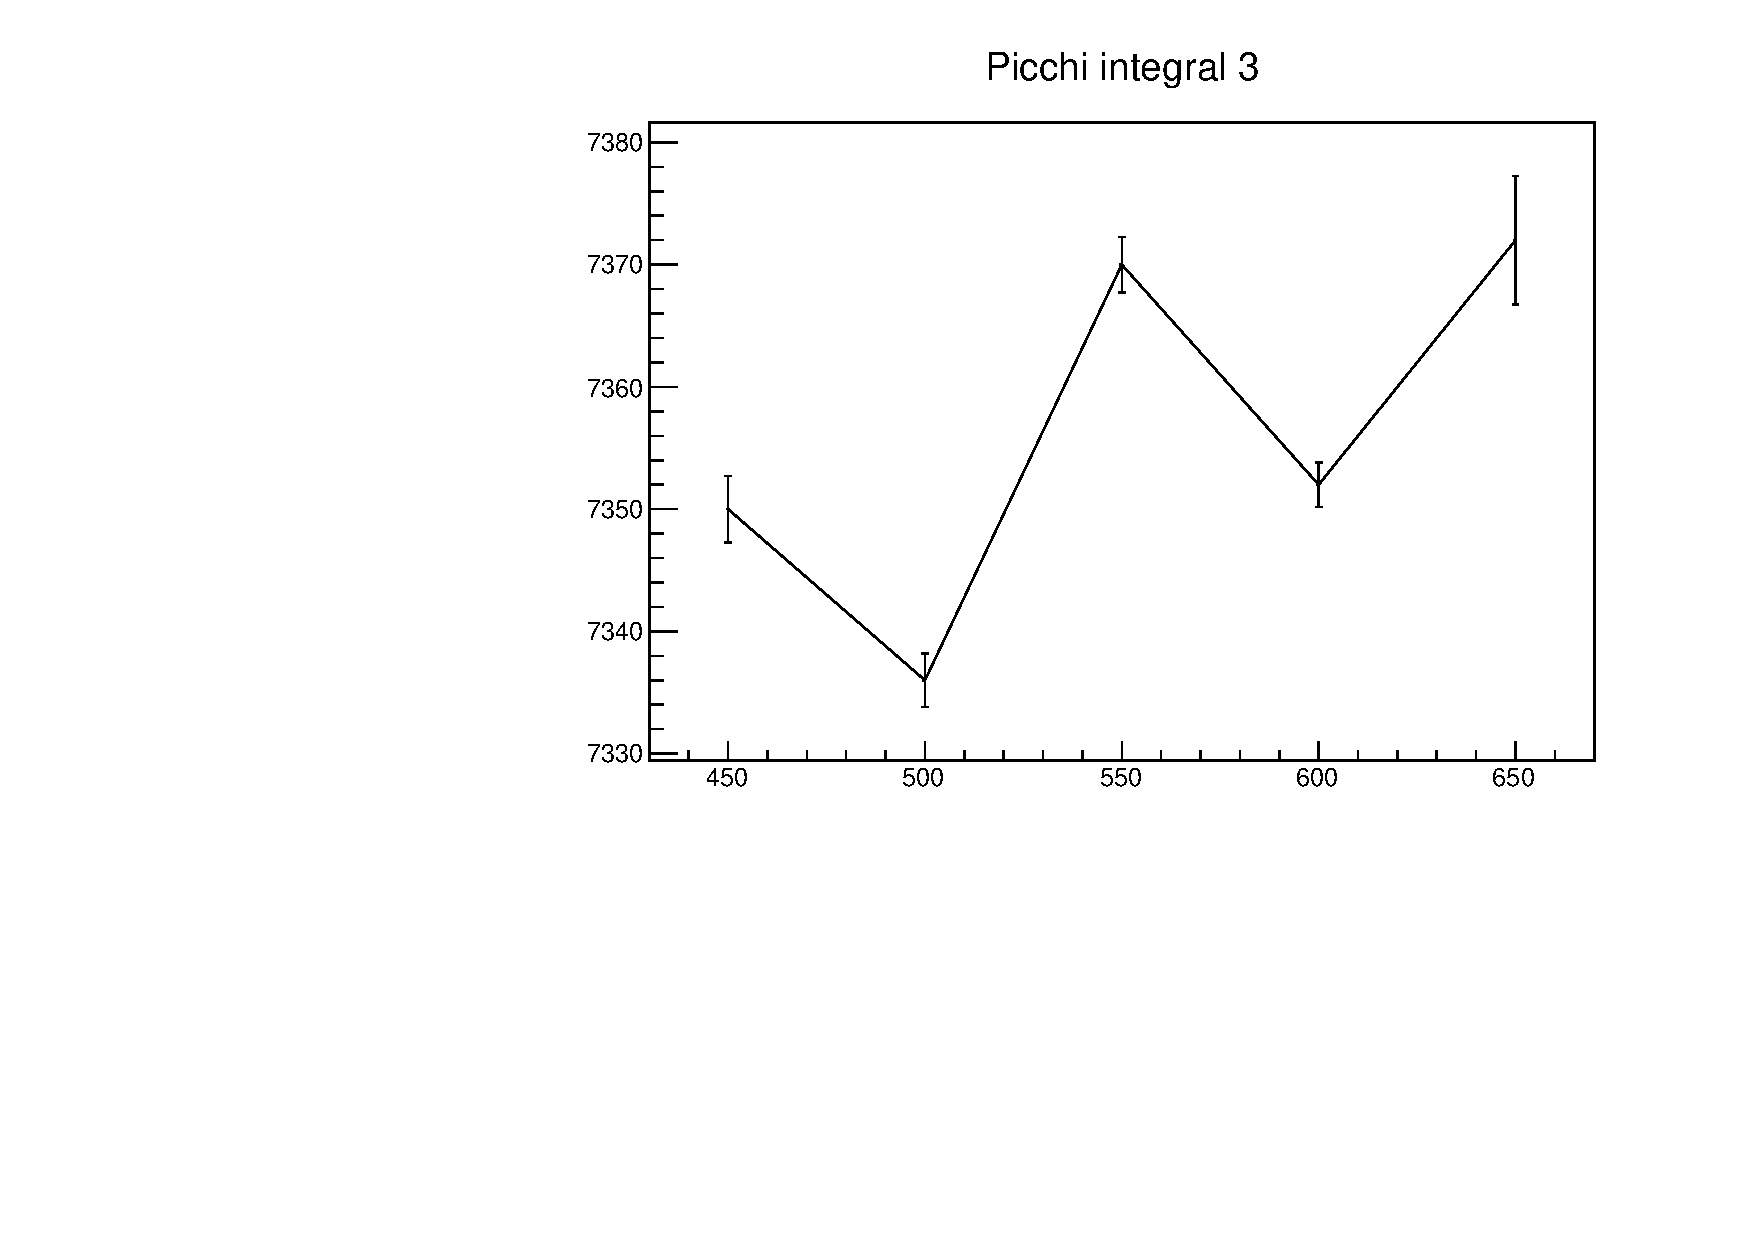
\includegraphics{../grafici/risultati/picchi_integral3.pdf}
 }%
 \caption{Andamento integrale del picco 3 in funzione della pressione [mb]} 
 \label{gr:picchi_int3} 
\end{grafico}

\begin{grafico}
 \centering
 \resizebox{\textwidth}{!}{%
 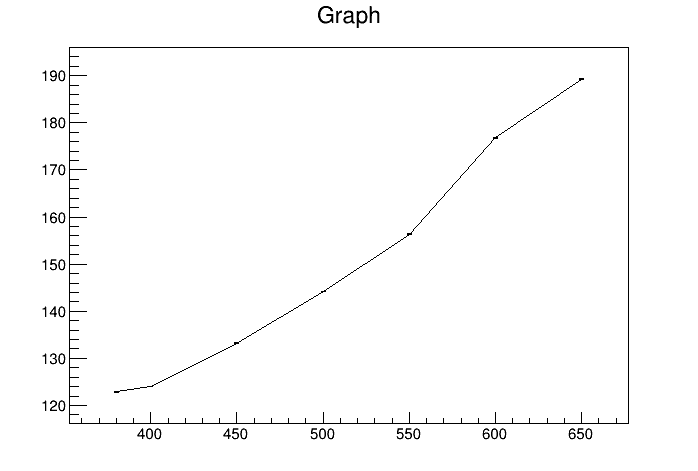
\includegraphics{../grafici/risultati/picchi_vmax.png}
 }%
 \caption{Andamento integrale di vmax [V] in funzione della pressione [mb]} 
 \label{gr:picchi_vmax} 
\end{grafico}

Come si può vedere dai grafici TODO INSERIRE LABEL QUI, l'integrale dei picchi, ovvero l'energia della particella alfa, rimane costante al variare della pressione,
almeno finche non si arriva a pressioni troppo basse. Questo cambiamento a pressioni basse è dovuto al fatto che a bassa pressione le particelle riescono ad arrivare oltre la lunghezza della camera, e la restante carica non viene più rivelata.
Addirittura, il terzo picco sparisce a basse pressioni, confondendosi con il secondo a causa dell'energia mancante.

Nel grafico di vmax invece si può chiaramente notare un andamento lineare (TODO perché?).

\FloatBarrier